%%%%%%%%%%%%%%%%%%%%%%%%%%%%%%%%%%%%%%%%%%%%%%%%%%%%%%
% A Beamer template for University of Wollongong     %
% Based on THU beamer theme                          %
% Author: Qiuyu Lu                                   %
% Date: July 2024                                    %
% LPPL Licensed.                                     %
%%%%%%%%%%%%%%%%%%%%%%%%%%%%%%%%%%%%%%%%%%%%%%%%%%%%%%
% Customized for Sharif University of Technology     %
%%%%%%%%%%%%%%%%%%%%%%%%%%%%%%%%%%%%%%%%%%%%%%%%%%%%%%


\documentclass[default, aspectratio=169]{beamer}
%\documentclass[default]{beamer}  % for 4:3 ratio
\usepackage[T1]{fontenc} 
\usepackage{fourier-otf} % see "http://faq.ktug.org/wiki/uploads/MathFonts.pdf" for other options
\usepackage{hyperref}
\usepackage{latexsym,amsmath,xcolor,multicol,booktabs,calligra}
\usepackage{graphicx,pstricks,listings,stackengine}
\usepackage{lipsum}
\usepackage{tikz}
\usepackage{pgffor}


\author{Ali Sharifi-Zarchi}
\title{Machine Learning (CE 40717)}
\subtitle{Fall 2024}
\institute{
	CE Department \\
	Sharif University of Technology
}
%\date{\small \today}
% \usepackage{UoWstyle}
\usepackage{SUTstyle}
\usepackage{amsmath}
\usepackage{amssymb}

%\usepackage{multicol}

% defs
\def\cmd#1{\texttt{\color{red}\footnotesize $\backslash$#1}}
\def\env#1{\texttt{\color{blue}\footnotesize #1}}
\definecolor{deepblue}{rgb}{0,0,0.5}
\definecolor{deepred}{RGB}{153,0,0}
\definecolor{deepgreen}{rgb}{0,0.5,0}
\definecolor{halfgray}{gray}{0.55}

\lstset{
	basicstyle=\ttfamily\small,
	keywordstyle=\bfseries\color{deepblue},
	emphstyle=\ttfamily\color{deepred},    % Custom highlighting style
	stringstyle=\color{deepgreen},
	numbers=left,
	numberstyle=\small\color{halfgray},
	rulesepcolor=\color{red!20!green!20!blue!20},
	frame=shadowbox,
}

\begin{document}
	
	
	
	\begin{frame}
		\titlepage
		\vspace*{-0.6cm}
		\begin{figure}[htpb]
			\begin{center}
				
\includegraphics[keepaspectratio, scale=0.25]{pic/sharif-main-logo.png}
			\end{center}
		\end{figure}
	\end{frame}
	
	\begin{frame}    
		\tableofcontents[sectionstyle=show,
		subsectionstyle=show/shaded/hide,
		subsubsectionstyle=show/shaded/hide]
	\end{frame}
	\section{Channels}
	
	\begin{frame}{Channels}
		Previously, we discussed 2D inputs; however, although images are inherently 2D, they need to be represented as \textbf{3D matrices} to display color information.
		\newline
		\begin{itemize}
			\item Pixel values range from 0 to 255.
			\item It is not possible to represent all the colors in a picture using only a single channel of numbers from 0 to 255.
			\item Thus, we represent them using \textbf{three channels}.
		\end{itemize}
		\centering
		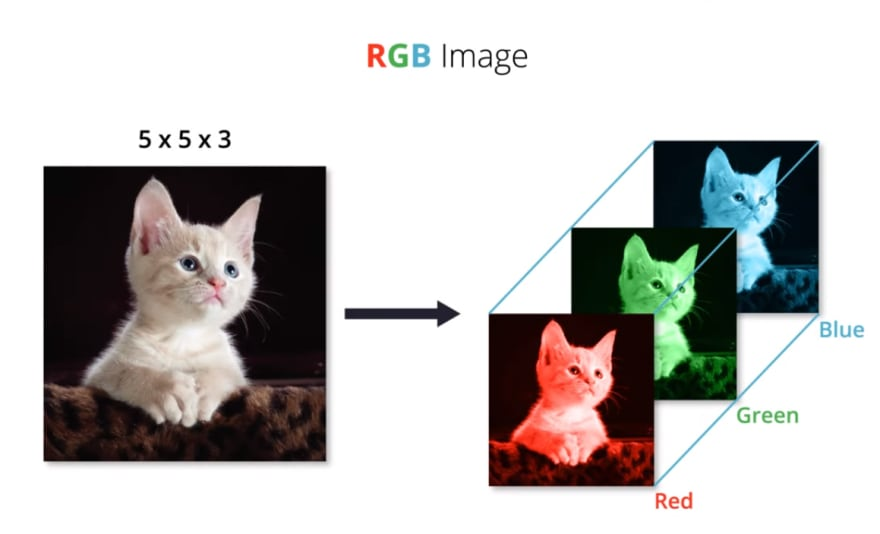
\includegraphics[keepaspectratio, scale=0.2]{pic/channels1.jpeg}
		
		\vfill
		\begin{tikzpicture}[remember picture,overlay]
			\node[anchor=south west, xshift=0.5cm, yshift=0.5cm] at (current page.south west) {
				\scriptsize Figure adapted from \href{https://dev.to/sandeepbalachandran/machine-learning-going-furthur-with-cnn-part-2-41km}{Source}
			};
		\end{tikzpicture}
	\end{frame}
	
	\begin{frame}{Channels}
		\begin{center}
			\begin{figure}
				\centering
				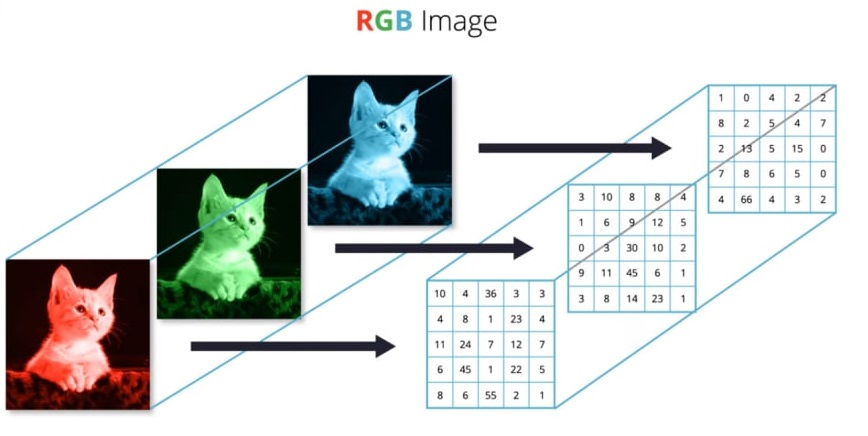
\includegraphics[keepaspectratio, scale=0.6]{pic/channels2.jpeg}
				\vfill
				\begin{tikzpicture}[remember picture,overlay]
					\node[anchor=south west, xshift=0.5cm, yshift=0.5cm] at (current page.south west) {
						\scriptsize Figure adapted from \href{https://dev.to/sandeepbalachandran/machine-learning-going-furthur-with-cnn-part-2-41km}{Source}
					};
				\end{tikzpicture}
			\end{figure}
		\end{center}
	\end{frame}
	
	
	\begin{frame}{Channels}
		\begin{itemize}
			\item Each filter produces \textbf{one output channel}. By applying multiple filters, we can create multiple output channels, allowing each channel to learn \textbf{distinct} features.
		\end{itemize}
		
		\begin{center}
			\begin{figure}
				\centering
				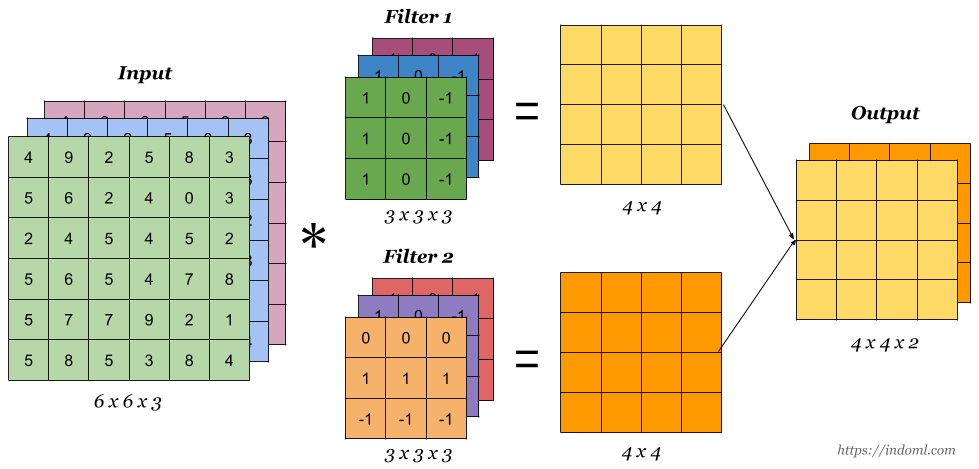
\includegraphics[width=0.7\columnwidth]{pic/channels5.png}
				\vfill
				\begin{tikzpicture}[remember picture,overlay]
					\node[anchor=south west, xshift=0.5cm, yshift=0.5cm] at (current page.south west) {
						\scriptsize Figure adapted from \href{https://indoml.com/2018/03/07/student-notes-convolutional-neural-networks-cnn-introduction/}{Source}
					};
				\end{tikzpicture}
			\end{figure}
		\end{center}
	\end{frame}
	
	
	\begin{frame}
		\large \centering
		\textbf{Let's take a closer look at the calculations} 
	\end{frame}
	
	\foreach \i in {1,...,18}
	{
		\begin{frame}{Channels}
			\begin{figure}
				\centering
				\includegraphics[width=0.45\columnwidth]{pic/cs231n-conv-\i.png}        
				\vfill
				\begin{tikzpicture}[remember picture,overlay]
					\node[anchor=south west, xshift=0.5cm, yshift=0.5cm] at (current page.south west) {
						\scriptsize Figure adapted from [2]
					};
				\end{tikzpicture}
			\end{figure}
		\end{frame}
	}
	\section{Pooling}
	\begin{frame}{Review}
		\textbf{Three Main Types of Layers}
		\begin{itemize}
			\item \textbf{Convolutional Layer}
			\begin{itemize}
				\item Neurons' outputs are connected to local regions in the input.
				\item Applying the same filter across the entire image.
				\item The parameters of the CONV layer include a set of learnable filters.
			\end{itemize}
			\item \textbf{Pooling Layer}
			\begin{itemize}
				\item Performs a downsampling operation along the spatial dimensions.
			\end{itemize}
			\item \textbf{Fully-Connected Layer}
			\begin{itemize}
				\item Typically used in the final stages of the network for combining high-level features to make predictions.
			\end{itemize}
		\end{itemize}
	\end{frame}
	\begin{frame}{Pooling}
		\begin{itemize}
			\item Convolution and activation layers are often followed by pooling layers intermittently.
			
			\begin{itemize}
				\item Pooling layers often alternate with convolution layers, although this is not mandatory.
			\end{itemize}
		\end{itemize}
		\centering
		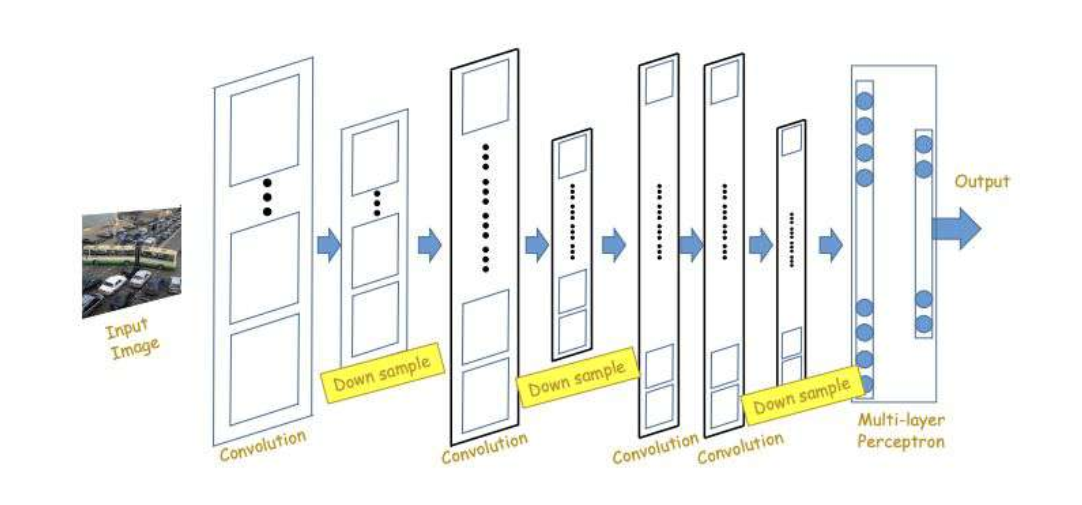
\includegraphics[keepaspectratio, scale=0.5]{pic/pooling.png}
	\end{frame}
	\begin{frame}{Pooling}
		\begin{minipage}{0.4\textwidth}
			\centering
			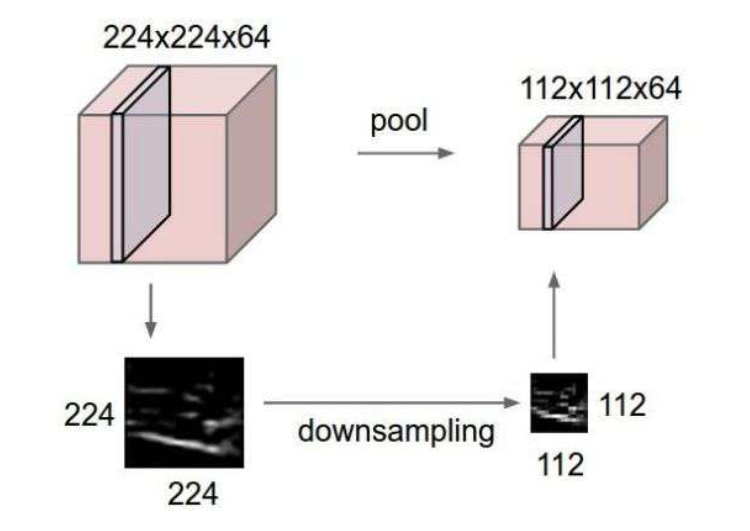
\includegraphics[keepaspectratio, scale=0.4]{pic/pooling1.png}
		\end{minipage}%
		\hspace{0.5cm}  % Adjust spacing as needed
		\begin{minipage}{0.55\textwidth}
			\smallskip
			\begin{itemize}
				\item Reduces the \textbf{spatial size} of the representation.
				\begin{itemize}
					\item To reduce the number of parameters and computational demands within the network.
					\item To \textbf{reduce variability}.
				\end{itemize}
				\item Enables the network to be invariant to small translations or distortions.
			\end{itemize}
		\end{minipage}
		\vfill
		\begin{tikzpicture}[remember picture,overlay]
			\node[anchor=south west, xshift=0.5cm, yshift=0.5cm] at (current page.south west) {
				\scriptsize Figure adapted from [2]
			};
		\end{tikzpicture}
	\end{frame}
	\begin{frame}{Pooling Type}
		\centering
		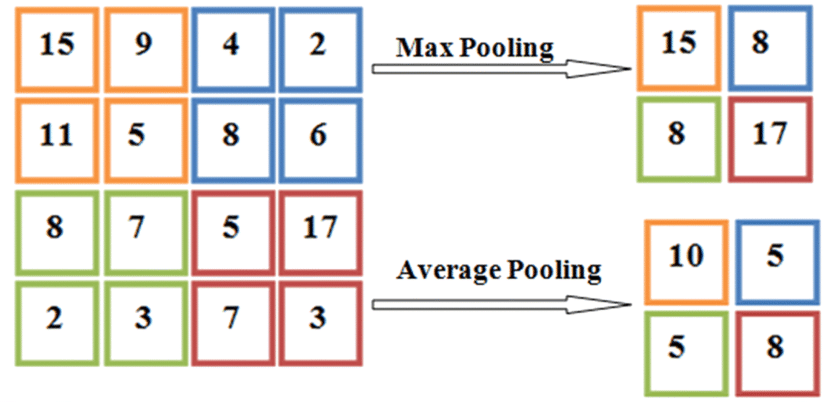
\includegraphics[keepaspectratio, scale=0.5]{pic/pooling2.png}
		\begin{flushleft}
			\textbf{Two Primary Types of Pooling:}
			\begin{itemize}		
				\item \textbf{Max Pooling:}  \small Selects the \textbf{maximum} value from each section of the feature map.
				\item \textbf{Min Pooling:}  \small Selects the \textbf{minimum} value from each section of the feature map.
				\item \textbf{Average Pooling:} \small Calculates the \textbf{average} value for each section of the feature map.
			\end{itemize}
			
			\vfill
			\begin{tikzpicture}[remember picture,overlay]
				\node[anchor=south west, xshift=0.5cm, yshift=0.5cm] at (current page.south west) {
					\scriptsize Figure adapted from \href{https://www.researchgate.net/figure/Two-common-types-of-pooling-method_fig1_355406505}{source}
				};
			\end{tikzpicture}
		\end{flushleft}
	\end{frame}
	\begin{frame}{Pooling Type}
		\begin{itemize}
			\item Max Pooling works well \textbf{when the background is light}, and the object is dark.
			\item Min Pooling works well \textbf{when the background is dark}, and the object is light.
			\item Average Pooling: \textbf{smooths} the feature map.
		\end{itemize}
		
		\centering
		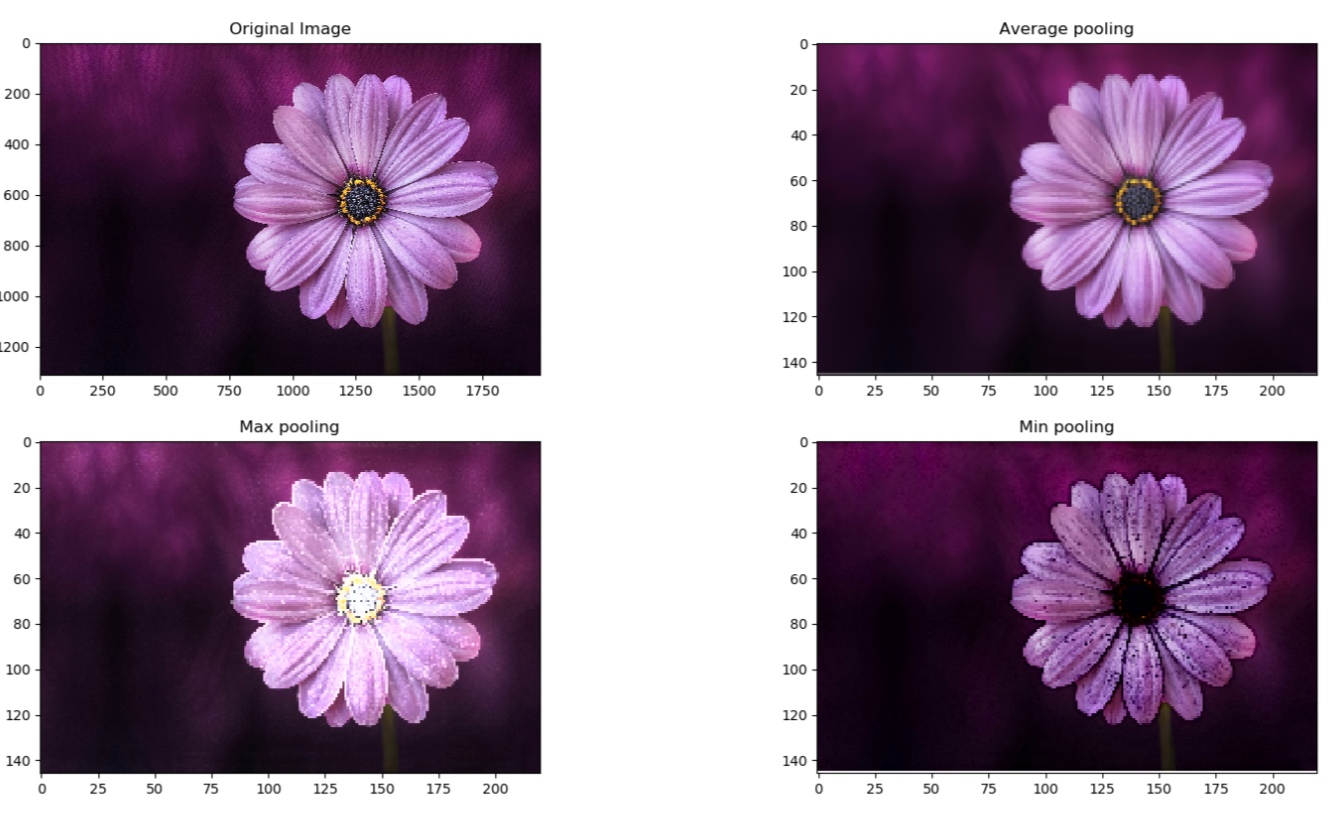
\includegraphics[keepaspectratio, scale=0.15]{pic/Pooling_3.png}
	\end{frame}
	\begin{frame}{Max Pooling}
		
		\centering
		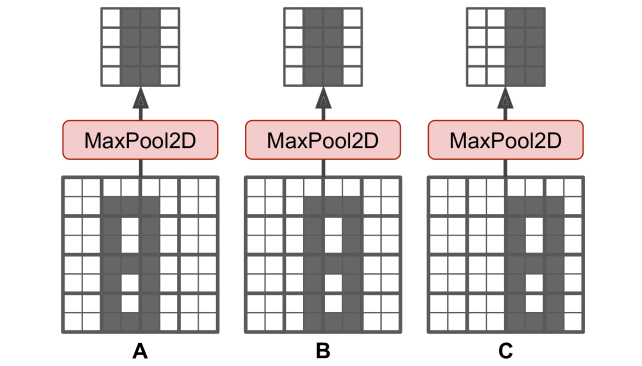
\includegraphics[keepaspectratio, scale=0.3]{pic/Pooling_4.png}
		\bigskip
		\begin{itemize}
			\item This is the most common type of pooling layer.
			\item Provides invariance to small translations.
		\end{itemize}
		
	\end{frame}
	\begin{frame}{Parameter Setting}
		\textbf{Question:} \\
		How does a pooling layer change the input image dimensions?
		
		\bigskip
		
		\textbf{Answer:} \\
		\begin{itemize}
			\item An $N \times N$ image, when compressed by a $P \times P$ pooling filter with a stride of $S$, produces an output map with side length $\left\lceil \frac{(N - P)}{S} \right\rceil + 1$.
			
		\end{itemize}
	\end{frame}
	\begin{frame}{Parameter Setting}
		\begin{itemize}
			\item Pooling takes in a volume of size $W_1 \times H_1 \times D_1$
			\item Requires two hyperparameters:
			\begin{itemize}
				\item Their spatial extent $P$,
				\item The stride $S$.
			\end{itemize}
			\item Produces an output volume of size $W_2 \times H_2 \times D_2$, where:
			\begin{itemize}
				\item $W_2 = \frac{(W_1 - P)}{S} + 1$
				\item $H_2 = \frac{(H_1 - P)}{S} + 1$
				\item $D_2 = D_1$
			\end{itemize}
			\item Introduces \textbf{zero parameters} since it computes a fixed function of the input.
			\item Using zero-padding for pooling layers is \textbf{uncommon}.
		\end{itemize}
	\end{frame}
	\begin{frame}{Downsampling}
		\centering
		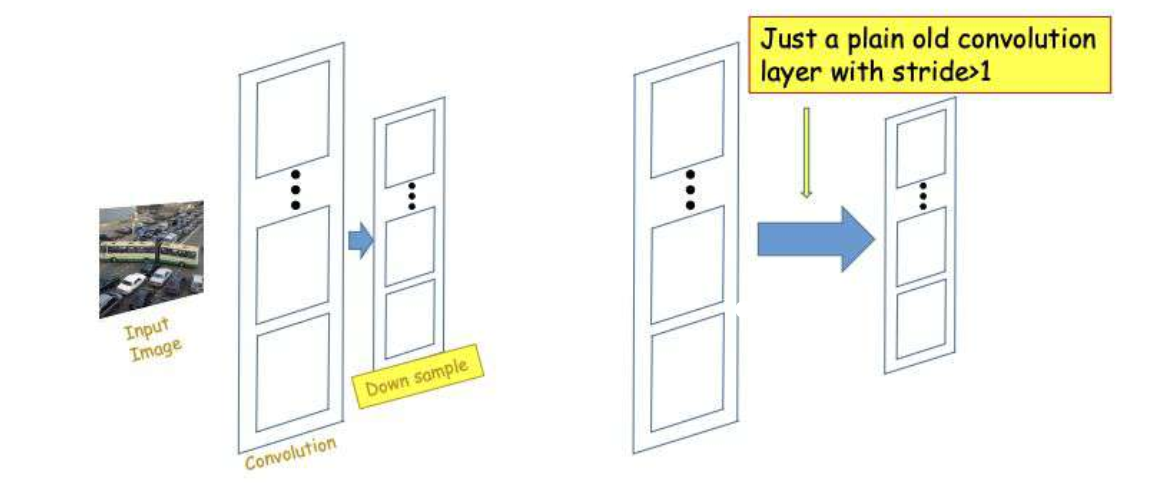
\includegraphics[keepaspectratio, scale=0.55]{pic/pooling3.png}
		\smallskip
		\begin{itemize}
			\item Downsampling can be done by a simple convolution layer with stride larger than 1, Replacing the max pooling layer with a convolutional layer.
		\end{itemize}
		
	\end{frame}
	\begin{frame}{Pooling Summary}
		\begin{minipage}{0.5\textwidth}
			\centering
			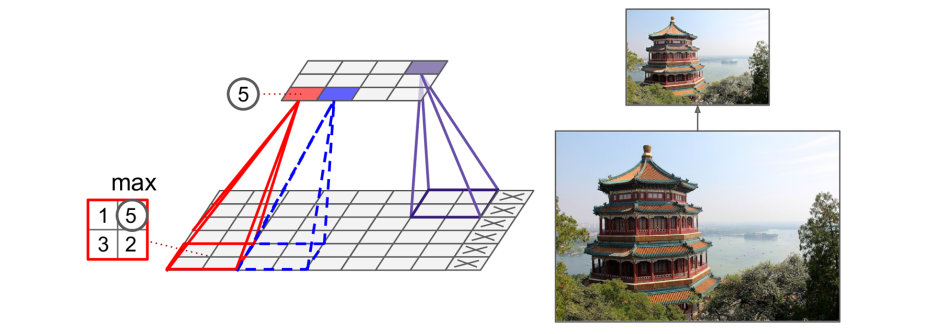
\includegraphics[keepaspectratio, scale=0.25]{pic/Pooling_2.png}
			
			\vspace{0.3cm}
			\small Max pooling layer (2 $\times$ 2 kernel, stride 2, no padding)
		\end{minipage}%
		\hspace{0.4cm}  % Adjust horizontal space between the columns if needed
		\begin{minipage}{0.45\textwidth}
			\begin{itemize}
				\item The goal is to sub-sample the input to reduce:
				\begin{itemize}
					\item Computational load
					\item Memory usage
					\item Number of parameters
					\item Risk of overfitting
				\end{itemize}
			\end{itemize}
		\end{minipage}
	\end{frame}
	\begin{frame}{Question}
		\centering
		\begin{itemize}
			\centering
			\item \Large \textbf{What if we want to increase the dimensions?}
		\end{itemize}
	\end{frame}
	\begin{frame}{Up-sampling CNN}
		\vspace{0.5cm}
		\begin{itemize}
			\item Resizing feature maps is a \textbf{common} operation in neural networks, especially those used for image segmentation tasks.
			\item This architecture is often referred to as an \textbf{Encoder-Decoder} network.
		\end{itemize}
		\bigskip
		\centering
		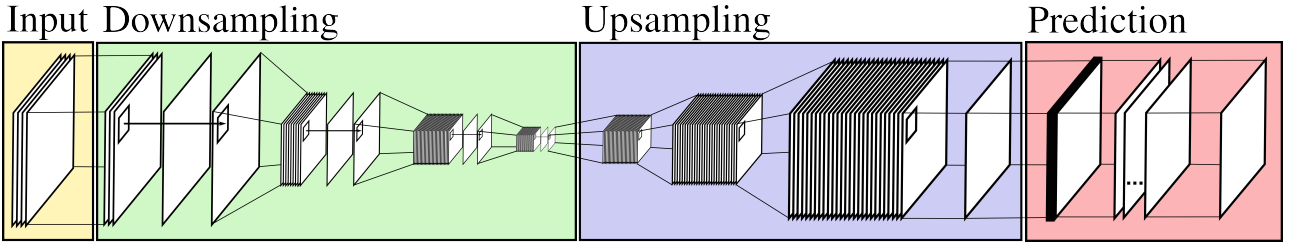
\includegraphics[keepaspectratio, scale=0.2]{pic/Upsamlpe_0.png}
		
	\end{frame}
	\begin{frame}{Nearest Neighbors}
		\vspace{0.5cm}
		\begin{itemize}
			\item \textbf{Nearest Neighbors}: Nearest Neighbors involves copying an input pixel value to the K-nearest neighboring pixels, with $K$ based on the expected output.
		\end{itemize}
		
		\centering
		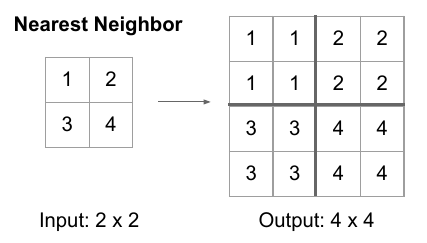
\includegraphics[keepaspectratio, scale=0.4]{pic/Upsamlpe_1.png}
	\end{frame}
	\begin{frame}{Bilinear Interpolation}
		\vspace{0.5cm}
		\begin{itemize}
			\item \textbf{Bilinear Interpolation}: In Bilinear Interpolation, the four nearest pixel values are used to compute a weighted average based on their distances, resulting in a smoothed output.
		\end{itemize}
		
		\centering
		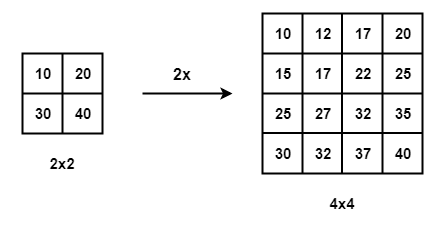
\includegraphics[keepaspectratio, scale=0.4]{pic/Upsamlpe_2.png}
		
	\end{frame}
	\begin{frame}{Bed Of Nails}
		\vspace{0.5cm}
		\begin{itemize}
			\item \textbf{Bed Of Nails}: In this method, the input pixel value is copied to the corresponding position in the output image, with zeros filling the remaining positions.
		\end{itemize}
		
		\centering
		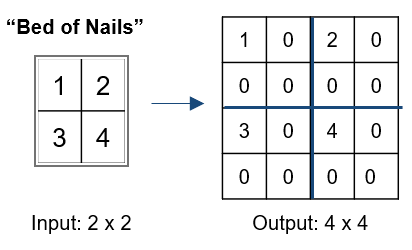
\includegraphics[keepaspectratio, scale=0.4]{pic/Upsamlpe_3.png}
		
	\end{frame}
	\begin{frame}{Max-Unpooling}
		\vspace{0.5cm}
		\begin{itemize}
			\item \textbf{Max-Unpooling}: In max-unpooling, the index of the \textbf{maximum value} is saved for each max-pooling layer during encoding. During decoding, the saved index is used to map the input pixel to its original position, with zeros filling all other positions.
		\end{itemize}
		
		\centering
		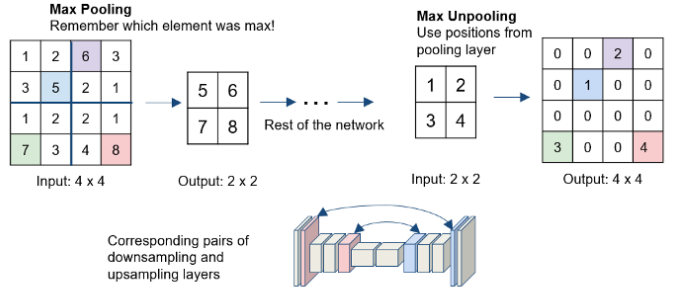
\includegraphics[keepaspectratio, scale=0.3]{pic/Upsamlpe_4.png}
	\end{frame}
	
	
	
	
	
	
	\begin{frame}{Backpropagation With Pooling Layers}
		\large
		In our previous discussions, we explored the process of backpropagation in CNNs without considering pooling layers. Now, let's discuss how to adapt our algorithm to include pooling layers.
		
		\begin{itemize}
			\item 	The primary task is to handle the gradients effectively during backpropagation through pooling layers.
			\item In both cases, the gradients from the next layer are \textbf{passed back} to the previous layer through the pooling operation.
			
		\end{itemize}
	\end{frame}
	
	\begin{frame}{Case 1}
		\centering
		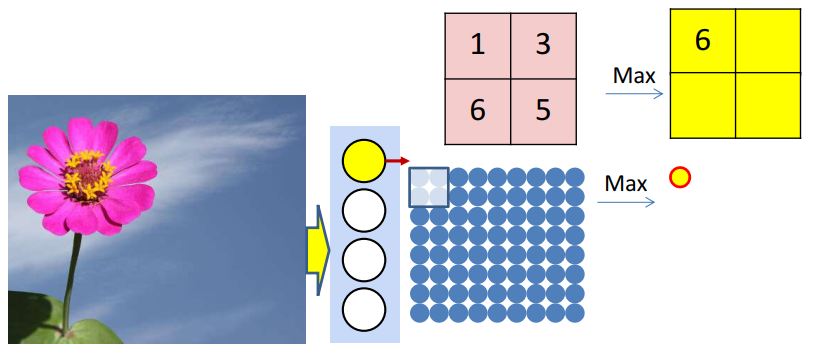
\includegraphics[keepaspectratio, scale=0.7]{pic/pconv1.png}
	\end{frame}
	
	\begin{frame}{Case 1}
		For \textbf{Max Pooling:}
		\begin{itemize}
			\item The gradient is propagated only through the \textbf{indices of the maximum values} identified during the forward pass.
			\item All other positions receive a gradient of \textbf{zero}.
		\end{itemize}
		\centering
		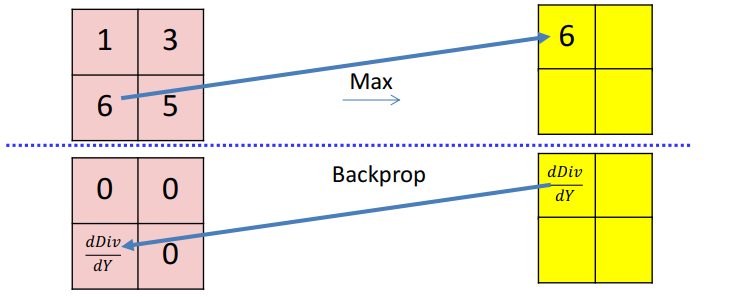
\includegraphics[keepaspectratio, scale=0.5]{pic/pconv2.png}
	\end{frame}
	
	\begin{frame}{Case 2}
		\centering
		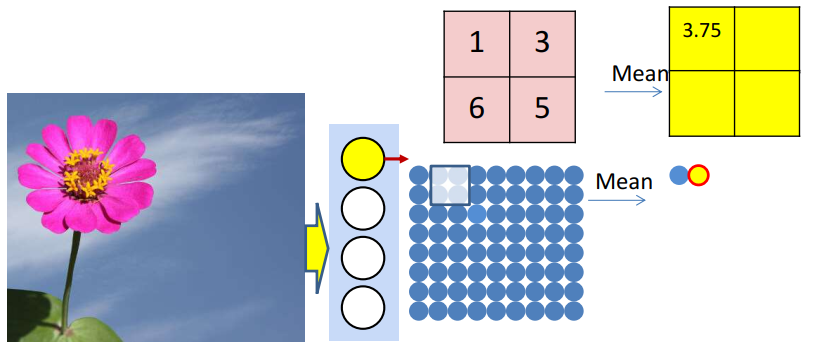
\includegraphics[keepaspectratio, scale=0.7]{pic/pconv3.png}
	\end{frame}
	
	\begin{frame}{Case 2}
		For \textbf{Average Pooling:}
		\begin{itemize}
			\item The gradients are \textbf{uniformly distributed} across the pooled region.
		\end{itemize}
		\centering
		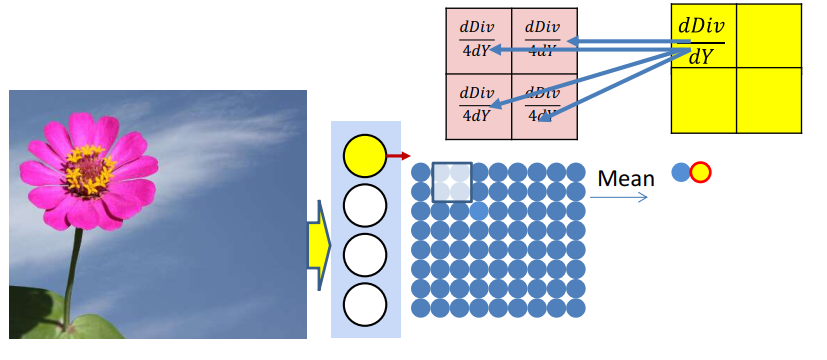
\includegraphics[keepaspectratio, scale=0.5]{pic/pconv4.png}
	\end{frame}
	
	
	
	\section{Receptive field \& inductive bias}
	
	\begin{frame}{Receptive Field}
		\centering
		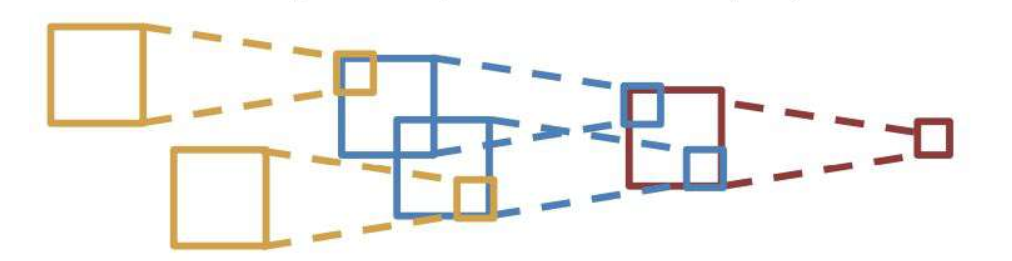
\includegraphics[keepaspectratio, scale=0.6]{pic/receptive1.png}
		\smallskip
		\begin{itemize}
			\item \textbf{Receptive Field:} How large is the region in the \textbf{input or previous layer} seen by a neuron on the n-th convolutional layer?
			\item In a convolution with kernel size $K$, each element in the next layer is based on a $K \times K$ \textbf{receptive field} from the previous layer.
		\end{itemize}
		\vfill
		\begin{tikzpicture}[remember picture,overlay]
			\node[anchor=south west, xshift=0.5cm, yshift=0.5cm] at (current page.south west) {
				\scriptsize Figure adapted from [3]
			};
		\end{tikzpicture}
	\end{frame}	
	\begin{frame}{Receptive Field}
		\centering
		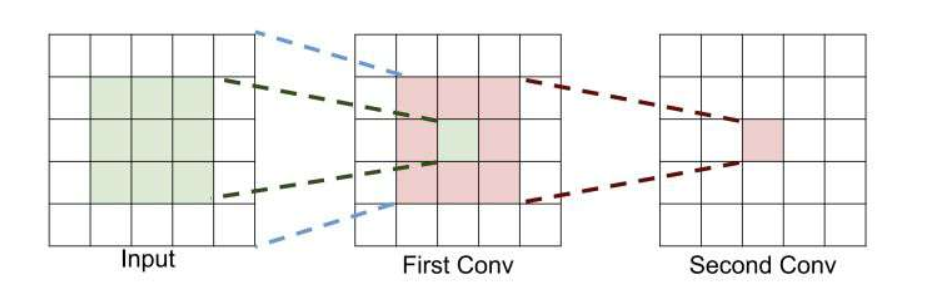
\includegraphics[keepaspectratio, scale=0.6]{pic/receptive.png}
		\smallskip
		\begin{itemize}
			\item Units in the deeper layers can be \textbf{indirectly} connected to most of the input image.
			\item Each successive convolution adds $K - 1$ to the receptive field size. With $L$ layers, the receptive field size is $1 + L \cdot (K - 1)$.
			\item \textbf{Challenge}: For large images, many layers are required for each output to capture the entire image.
			\begin{itemize}
				\item \textbf{Solution:} \textbf{Downsample} within the network using strides and pooling layers.
			\end{itemize}
		\end{itemize}
	\end{frame}
	\begin{frame}{Power Of Small Filters}
		Assuming an input size of  $H \times W \times C$, and convolutions are used with $C$ filters to preserve depth (stride 1, with padding to maintain $H$ and $W$ dimensions).
		
		\bigskip
		\begin{minipage}{0.45\textwidth}
			\textcolor{blue}{\textbf{one CONV with 7 x 7 filters}} \\
			Number of weights \\
			$= C \times (7 \times 7 \times C) = \textbf{49} C^2$
		\end{minipage}
		\hfill
		\begin{minipage}{0.45\textwidth}
			\textbf{three CONV with 3 x 3 filters} \\
			Number of weights \\
			$= 3 \times C \times (3 \times 3 \times C) = \textbf{27} C^2$
		\end{minipage}
		\bigskip
		\begin{flushleft}
			Both options achieve a receptive field of 7. However, using \textbf{multiple smaller filters} reduces the number of \textbf{parameters}, introduces more \textbf{nonlinearity}, and generally leads to a \textbf{more efficient}, expressive model.
		\end{flushleft}
	\end{frame}	
	\begin{frame}{Question}
		\textbf{Question:} In a convolutional neural network, each layer increases the receptive field size. 
		Suppose a network has 3 convolutional layers, each with a kernel size of \( K = 3 \) and a stride of \( S = 1 \).
		\begin{itemize}
			\item Determine the receptive field size after each layer, beginning with an initial receptive field size of \( 1 \).
			\item How large is the receptive field after the third layer?
			\item Why is the growing receptive field important in deeper layers?
		\end{itemize}
	\end{frame}
	
	\begin{frame}{Answer}
		\textbf{Answer:}
		\begin{itemize}
			\item The receptive field size increases by \( K - 1 \) with each layer.
			\begin{itemize}
				\item After the 1st layer: \( 1 + (3 - 1) = 3 \)
				\item After the 2nd layer: \( 3 + (3 - 1) = 5 \)
				\item After the 3rd layer: \( 5 + (3 - 1) = 7 \)
			\end{itemize}
			\item Consequently, the receptive field size after the third layer is \( 7 \).
			\item A larger receptive field allows neurons in deeper layers to capture more context from the input, crucial for recognizing higher-level patterns.
		\end{itemize}
	\end{frame}
	\begin{frame}{Inductive Bias In CNNs}
		\textbf{Inductive Bias:} \\
		The assumptions a model uses to generalize from training data to new, unseen data.
		
		\bigskip
		\textbf{Key Features of Inductive Bias in CNNs:}
		\begin{itemize}
			\item \textbf{Weight Sharing:} \\
			A single filter is applied across various regions of the input, significantly decreasing the parameter count.
			
			\item \textbf{Locality:} \\
			CNNs utilize small filters (e.g., $3 \times 3$) that concentrate on local regions, aligning well with image data where local structures are significant.
			
			\item CNNs are more sample-efficient than FCNs due to their inductive biases.
		\end{itemize}
	\end{frame}
	
	
	\section{References}
	\begin{frame}{Contributions}
		\begin{itemize}
			\item \textbf{This slide was prepared with contributions from:}
			\begin{itemize}
				\setlength{\itemsep}{10pt}
				\item \href{https://github.com/Ali0281}{Ali Aghayari}
			\end{itemize}
		\end{itemize}
		
	\end{frame}
	
	\begin{frame}[allowframebreaks]
		\bibliography{ref}
		\bibliographystyle{ieeetr}
		\nocite{*}
	\end{frame}
	
	
\end{document}
